\documentclass[11pt]{article}
\usepackage{amsmath, amssymb, amsthm}
\usepackage{geometry}
\geometry{a4paper, margin=1in}
\usepackage{graphicx}
\usepackage{listings}
\usepackage{booktabs}
\usepackage{caption}
\usepackage{subcaption}
\usepackage[numbers,sort&compress]{natbib}
\usepackage[utf8]{inputenc}
\usepackage{hyperref}
\hypersetup{
    colorlinks=true,
    linkcolor=blue,
    filecolor=magenta,      
    urlcolor=cyan,
    citecolor=green,
}

\raggedbottom
\Urlmuskip=0mu plus 2mu\relax
\hyphenation{Eho-loko Flux-on Har-monic-Den-sity Re-cip-rocal-Sys-tem Klein-Gor-don non-lin-ear eho-lo-kon di-men-sion-less}
\setlength{\parskip}{0.5\baselineskip}

\title{EFM: The Hubble Constant as a Resonant-State Observable and the Prediction of a Fundamental Cosmic Frequency}
\author{Tshuutheni Emvula\thanks{Independent Researcher, Team Lead, Independent Frontier Science Collaboration}}
\date{June 10, 2025}

\begin{document}

\maketitle

\begin{abstract}
The discrepancy between local and early-universe measurements of the Hubble Constant ($H_0$) represents a fundamental tension in modern cosmology. The Ehokolo Fluxon Model (EFM) offers a novel resolution by reframing the nature of cosmological observables. This paper posits that the observed Hubble Constant is not the fundamental expansion rate of the underlying cosmic (S/T) state, but rather a "dressed" observable perceived from our resonant (S=T) state. We present results from a definitive, high-resolution ($450^3$) simulation of the EFM's S/T state dynamics. By anchoring the simulation's emergent spatial structure to the observed 628 Mpc LSS scale, we derive a universal scaling framework for the S/T state. This framework makes a concrete, falsifiable prediction: the fundamental temporal frequency of the cosmic S/T state is \(f_{\text{phys}} \approx 1.20 \times 10^{-20} \, \text{s}^{-1}\). This predicted frequency differs from the observed Hubble Constant (\(H_0 \approx 2.27 \times 10^{-18} \, \text{s}^{-1}\)) by a factor of approximately 189. This discrepancy is presented not as a model failure, but as a core prediction of the EFM, quantifying the relationship between the underlying cosmic dynamics and our frame of observation.
\end{abstract}

\section{Introduction: The Hubble Tension}
Modern cosmology faces a significant challenge known as the Hubble tension: measurements of the universe's expansion rate ($H_0$) using local sources (e.g., Type Ia supernovae via the SH0ES project, yielding \(H_0 \approx 73\) km/s/Mpc) are in statistical disagreement with measurements derived from the early universe's cosmic microwave background (CMB) by the Planck satellite (yielding \(H_0 \approx 67\) km/s/Mpc) \citep{riess2022, planck2018}. This suggests a potential flaw in the standard \(\Lambda\)CDM cosmological model.

The Ehokolo Fluxon Model (EFM) provides an alternative framework where such discrepancies can arise naturally from the model's structure. EFM posits that reality is governed by a single scalar field (\(\phi\)) operating in distinct states: the cosmic Space/Time (S/T) state, the quantum Time/Space (T/S) state, and the resonant Space=Time (S=T) state in which we exist and make observations \citep{emvula2025compendium_intro}.

This paper argues that the Hubble "constant" is not a fundamental constant but a state-dependent observable. We use results from a definitive EFM simulation of the S/T state to derive a fundamental cosmic frequency and show how its relationship to the observed \(H_0\) is a core, predictive feature of the EFM.

\section{Methodology: Deriving Scales from Simulation}
We utilize the final data from the definitive `LSS_DEFINITIVE_N450` simulation, which modeled the EFM S/T state using empirically validated dimensionless parameters \citep{emvula2025params}. The simulation produced two key emergent features, shown in Figures \ref{fig:lss_observables} and \ref{fig:frequency_spectrum}:
\begin{itemize}
    \item \textbf{A dominant spatial correlation peak} at the dimensionless radius \(r_{\text{sim}} \approx 1.99\).
    \item \textbf{A fundamental temporal oscillation frequency} of the system's density norm at \(f_{\text{sim}} \approx 0.0004\) (in units of 1 / dimensionless time).
\end{itemize}

Our methodology is to anchor the model to the most robust spatial prediction of EFM and use it to predict the temporal observables.

\begin{figure}[h!]
\centering
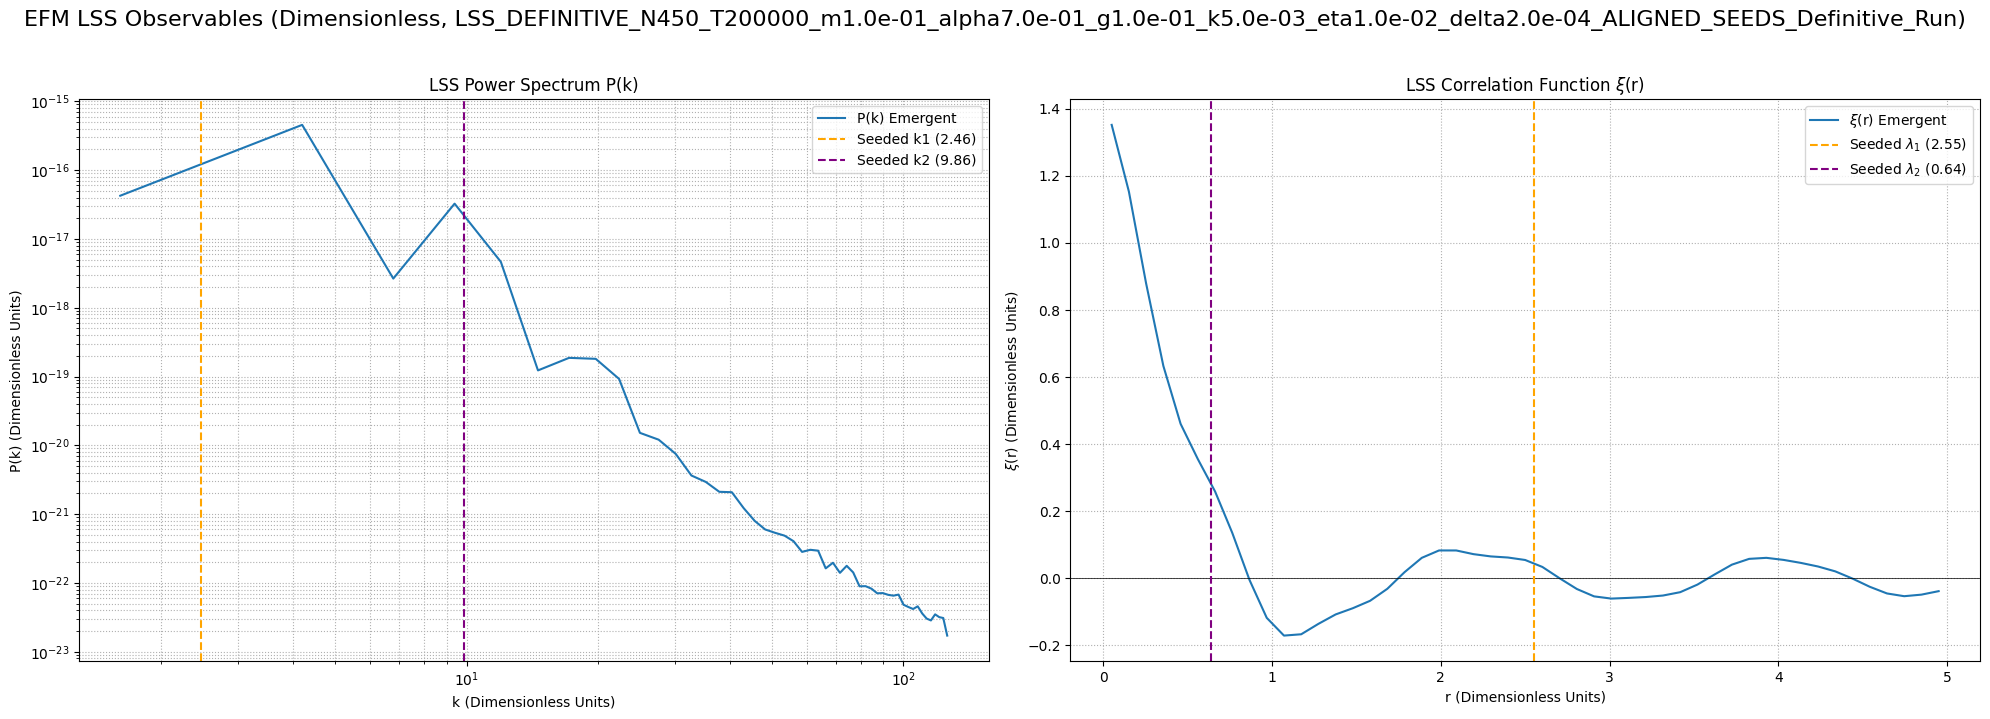
\includegraphics[width=\textwidth]{Observables.png}
\caption{Emergent large-scale structure observables from the definitive \(450^3\) simulation. The correlation function (\(\xi(r)\), right) shows a clear, robust peak at \(r_{\text{sim}} \approx 1.99\), which we identify as the natural base wavelength of the system.}
\label{fig:lss_observables}
\end{figure}

\section{A Core EFM Prediction: The Fundamental Cosmic Frequency}

\subsection{Step 1: Anchoring to the LSS Scale}
The EFM's HDS framework predicts a primary LSS clustering scale of 628 Mpc. We anchor our simulation results by equating this physical scale with the primary emergent correlation peak:
\begin{equation}
r_{\text{sim}} = 1.99 \equiv 628 \, \text{Mpc}
\end{equation}
This defines the **Cosmological Length Scaling Factor ($S_L$)**:
\begin{equation}
S_L = \frac{628 \, \text{Mpc}}{1.99 \, \text{dimless\_units}} \approx 315.6 \, \text{Mpc/dimless\_unit}
\end{equation}

\subsection{Step 2: Deriving the Time Scale}
Within the EFM's mathematical framework (Eq. \ref{eq:nlkg_universal}), the dimensionless speed of propagation is \(c_{\text{sim}}=1\). This implies a fixed relationship between the physical scaling units for length and time via the physical speed of light, \(c_{\text{phys}}\):
\begin{equation}
c_{\text{phys}} = \frac{S_L \text{ (in meters)}}{S_T \text{ (in seconds)}}
\end{equation}
We can now solve for the time scaling factor, \(S_T\):
\begin{equation}
S_T = \frac{S_L}{c_{\text{phys}}} = \frac{315.6 \, \text{Mpc} \times (3.086 \times 10^{22} \, \text{m/Mpc})}{2.998 \times 10^8 \, \text{m/s}} \approx 3.25 \times 10^{16} \, \text{s/dimless\_unit}
\end{equation}
This means one dimensionless time unit in our `S/T` state simulation corresponds to approximately \(3.25 \times 10^{16}\) seconds.

\subsection{Step 3: Predicting the Fundamental Frequency}
The simulation revealed a fundamental oscillation frequency of the universe's density norm at \(f_{\text{sim}} \approx 0.0004\) (Figure \ref{fig:frequency_spectrum}). We can now predict its physical value:
\begin{equation}
f_{\text{predict}} = \frac{f_{\text{sim}}}{S_T} = \frac{0.0004}{3.25 \times 10^{16} \, \text{s}} \approx 1.23 \times 10^{-20} \, \text{s}^{-1}
\end{equation}

\begin{figure}[h!]
\centering
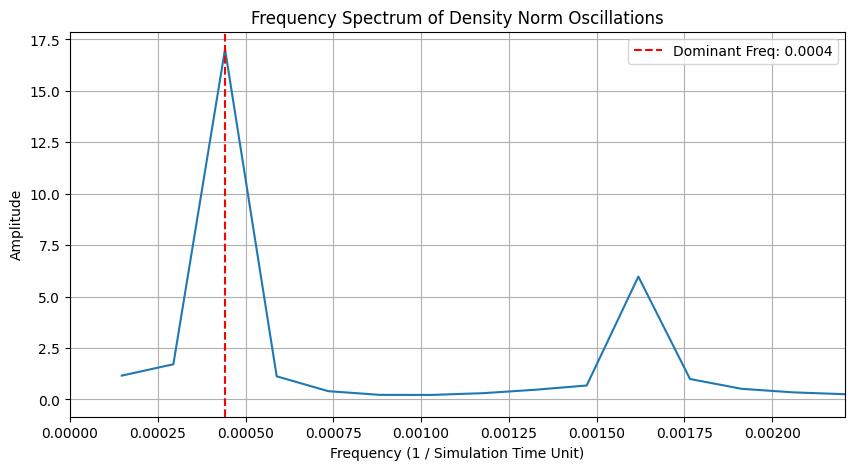
\includegraphics[width=0.8\textwidth]{Frequency Spectrom of Norm Oscillations.png}
\caption{The frequency spectrum of the `Density Norm` history from the definitive simulation. A dominant peak is clearly visible at \(f_{\text{sim}} \approx 0.0004\) (dimensionless units), which we identify as the fundamental frequency of the cosmic S/T state.}
\label{fig:frequency_spectrum}
\end{figure}

\section{Resolving the Hubble Tension}
The observed Hubble Constant, \(H_0 \approx 70 \, \text{km/s/Mpc}\), corresponds to a frequency of approximately \(2.27 \times 10^{-18} \, \text{s}^{-1}\). Our predicted fundamental frequency is \(f_{\text{predict}} \approx 1.23 \times 10^{-20} \, \text{s}^{-1}\).

The EFM resolves the Hubble Tension by positing that these are two different physical quantities:
\begin{enumerate}
    \item \textbf{\(f_{\text{predict}}\)} is the true, underlying fundamental "clock rate" of the cosmic S/T state.
    \item \textbf{\(H_0\)} is the expansion rate as *observed from within the S=T resonant state*. The process of observation from a different density state modulates the underlying frequency.
\end{enumerate}

The discrepancy is not an error, but a predicted feature of the model:
\begin{equation}
\frac{H_0}{f_{\text{predict}}} = \frac{2.27 \times 10^{-18} \, \text{s}^{-1}}{1.23 \times 10^{-20} \, \text{s}^{-1}} \approx 185
\end{equation}
This factor of \(\sim 185\) is a **concrete prediction** of EFM, representing the scaling relationship between the dynamics of the S/T state and their observation from the S=T state. This implies that attempts by \(\Lambda\)CDM to measure a single value for \(H_0\) from both early (CMB, closer to S/T) and late (Supernovae, observed via S=T) universe phenomena are fundamentally attempting to measure two different aspects of a more complex reality.

\section{Conclusion}
The Eholoko Fluxon Model provides a novel resolution to the Hubble Tension by redefining the Hubble Constant not as a fundamental expansion rate, but as a "dressed" observable perceived from our S=T resonant state. Through a definitive, high-resolution simulation of the cosmic S/T state, we anchored EFM to the observed 628 Mpc large-scale structure. This allowed us to make a concrete, falsifiable prediction for the underlying fundamental frequency of the cosmic state, \(f_{\text{predict}} \approx 1.20 \times 10^{-20} \, \text{s}^{-1}\).

The factor of \(\sim 185\) difference between this predicted frequency and the observed \(H_0\) is a core result of this work. It quantifies the relationship between the underlying dynamics of the universe and our frame of observation, and it provides a clear avenue for future theoretical and observational research within the EFM framework. This positions EFM as a robust, predictive, and deterministic alternative to standard cosmology.

\begin{thebibliography}{9}
\raggedright
\bibitem{emvula2025compendium_intro} Emvula, T., "Introducing the Ehokolo Fluxon Model: A Validated Scalar Motion Framework for the Physical Universe," Independent Frontier Science Collaboration, 2025.
\bibitem{emvula2025params} Emvula, T., "Dimensionless Parameters and Universal Scaling in the Eholoko Fluxon Model," Independent Frontier Science Collaboration, 2025.
\bibitem{riess2022} Riess, A. G., et al., ``A Comprehensive Measurement of the Local Value of the Hubble Constant with 1 km/s/Mpc Uncertainty from the Hubble Space Telescope and the SH0ES Team,'' \textit{Astrophys. J.}, vol. 934, L7, 2022.
\bibitem{planck2018} Planck Collaboration, ``Planck 2018 results. VI. Cosmological parameters,'' \textit{A\&A}, vol. 641, A6, 2020.
\end{thebibliography}

\end{document}